\documentclass[UTF8,10pt,a4paper,fontset=fandol]{ctexart}
\usepackage[margin=19mm]{geometry}
\usepackage{amsmath,graphicx,booktabs,tabularx,hyperref,float}
\hypersetup{hidelinks}
\setlength{\parindent}{2em}
\setlength{\parskip}{3pt}
\setlength{\textfloatsep}{10pt}
\setlength{\intextsep}{8pt}
\widowpenalty=10000
\title{因子流动性测试报告}\date{}\author{}
\begin{document}
{\Large\bfseries 因子流动性测试报告}\par
N20的扫板主情景在1000万元下，已定量的11,506笔合法订单全部在原日完成，但556个未知目标仍阻止容量认证；全期模型总收益率为-8.69\%；只完成1个资金档，资金衰减曲线尚未形成。

以上容量只检查事前合法订单；零计划、未建仓和取整造成的原目标差额另行披露，未知目标不算完成。

\begin{figure}[H]\centering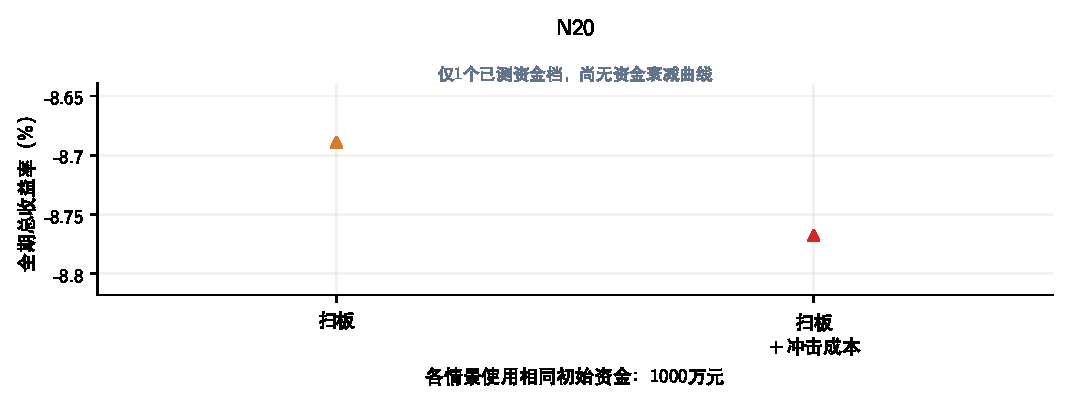
\includegraphics[width=\linewidth]{figures/capital_return.pdf}
\caption{本次只测1000万元，图中各点为同一资金档的不同执行情景。只展示全期完成并核账的结果；额外成本属于未校准的参数情景。}\end{figure}
\begin{table}[H]\centering\small\begin{tabular}{lllllr}\toprule 回看期 & 情景 & 最大已测通过 & 最低已测失败 & 通过档之上最近失败 & 已测档数\\\midrule N20 & 扫板 & 尚无 & 尚无 & 尚无 & 1 \\\bottomrule\end{tabular}\end{table}
“尚无通过档”不等于容量为零。表中每一档都对应实际测试；最近失败档和未测范围分别保留，连线不保证未测资金通过。

\subsection*{主情景各资金档状态}\begin{table}[H]\centering\small\begin{tabular}{lllrrrr}\toprule 回看期 & 情景 & 资金 & 总收益率 & 未完成订单 & 未知目标 & 判定\\\midrule N20 & 扫板 & 1000万元 & -8.69\% & 0 & 556 & 待核 \\\bottomrule\end{tabular}\end{table}

\section*{因子和实验设置}
本次输入因子：F000001收益率因子（N20含5\%扫板合法订单代表账户）。测试期为2024-01-02至2024-08-30。使用过去N个交易日复权价格变化的原始信号，经原批次预处理后取G1并等权配置。不同N只改变原回看期版本，不重选参数。

N表示因子的回看期，H表示调仓间隔，两者都按交易日计算。

N20：H=20，每20个交易日调仓；输入为已生成的目标持仓；沿用输入分组，取G1。

各资金档沿用同一套G1等权和H20规则。09:35先以账户净值乘目标权重、除参考价，减去实际持仓和应收权益，得到理论净需求，再按申报下限、增量和卖方整仓零股规则向下确定合法订单。舍入差额保留，不把资金或成交条件不足转成零目标。账户现金、持仓和权益连续保留到下一交易日。

本报告只展示初始资金为1000万元的代表账户，各情景分别连续回放；不据此推断其他资金规模的容量。

常规情景的成交量参与率为10\%。指令生效后，程序根据后续合格快照中观察到的新增成交量，逐步释放该股票的成交额度。同一股票的多笔订单共同使用这份额度，盘口中可见的对手方数量也会限制成交。此外，策略在该股的累计成交金额最多占截至当时市场已公布累计成交额的10\%。

扫板是本报告的主执行情景：距涨跌停幅度差1个百分点时触发，即上涨4\%／9\%／19\%或下跌4\%／9\%／19\%时均检查触发，对应5\%／10\%／20\%涨跌幅制度。触发后，假设后续合格观测产生的有效新增市场成交量全部可供本策略使用，买入按官方涨停价、卖出按官方跌停价记账。现金和可卖量仍受账户约束。本报告为另行定义的5\%／10\%／20\%扫板情景，不与原10\%／20\%基线混用。未启用额外冲击时不计该项成本；启用冲击的情景另列，均未模拟真实排队竞争。

本情景的通过条件是：测试期内，每笔事前确定的正数量合法订单均在计划当天100\%完成。合法计划量在09:35按理论净需求和申报数量规则确定，不按资金、可卖量、盘口或后来成交量缩小。非零订单未发出或仍有余量都未通过，后续成交不能修复原日失败。零合法计划单列目标偏差，不叫达成目标；全部为零而没有正合法订单的账户不能证明容量通过。资料不足的目标和账户仍待核。

本报告使用历史账户保存的跨日规则：当日未完成需求可在后续交易日按实际账户重新计算。这是本账户的历史执行行为，不是新订单的日终终止规则；后续成交始终不改写原日未完成结果。

\section*{未完成交易：数据、结果和原因}
已定量的合法订单均在原日完成。容量仍待确认的原因是下列未知目标，不能把它们改成零需求或已完成。图表用证券编号展示，实际股票代码和逐笔明细保存在私有结果目录。



每笔原始计划只计一次，后续记录不增加原日计划数。未知目标按正式评估的主原因归类，每个目标只归一类。其余执行证据可能重叠，各行数量不能相加，也不表示每种限制都直接导致了未成交。

主结果采用扫板，每个N优先展示最低未通过资金档，各账户分别列数。本节使用：N20/扫板 1000万元。其他情景见随附完整汇总。\subsection*{未知目标仍缺少的资料或政策}\begin{table}[H]\centering\small\begin{tabular}{lllr}\toprule 回看期 & 资金 & 保存的证据 & 计划数\\\midrule N20 & 1000万元 & 公司行动固定排除 & 522 \\
N20 & 1000万元 & 停牌起止时间不完整 & 15 \\
N20 & 1000万元 & 官方限价或特殊制度未核实 & 13 \\
N20 & 1000万元 & 决策前区间量额隐含价超界 & 3 \\
N20 & 1000万元 & 决策前最新状态为恢复基线 & 2 \\
N20 & 1000万元 & 决策前最新价格无效 & 1 \\\bottomrule\end{tabular}\end{table}\subsection*{盘中曾受限、但当日已完成}\begin{table}[H]\centering\small\begin{tabular}{lllr}\toprule 回看期 & 资金 & 保存的证据 & 计划数\\\midrule N20 & 1000万元 & 触发扫板假设 & 50 \\
N20 & 1000万元 & 记录过现金约束 & 4559 \\\bottomrule\end{tabular}\end{table}

缺少停牌的日内起止时间时，不能仅凭事件记录认定全天不能交易。

现金不足记录的是交易过程中曾遇到的限制；是否导致日终未完成，要结合对应订单的当日余量判断。

分红送转等权益处理与行情资料问题分别列出。缺少参考价、行情或交易状态时，先保留待核状态，补齐资料后再判断成交条件。参考价采用本报告账户保存的规则，正常无更新本身不证明数据损坏。

记录为关键事件排除的目标，按整个研究窗口的公司行动资料，在各账户共同现金起点固定排除。排除名单可能使用目标日之后才公告的事件资料，因此结果描述的是这一固定排除范围下的研究情景，不能解释为目标当日已知信息的筛选，也不表示当日缺少L2行情。涉及零碎股分配时，输入准备阶段按每股比例和来源分配要求统一判断，尚未结合各账户登记日的实际持股逐一判断应得新增股份是否恰为整数。原目标权重不重新分配，相关待核目标不计为成交完成。\section*{合法订单与权重目标偏差}本报告的100\%只指事前合法订单完成，不表示G1等权目标被100\%实现。G1成员、权重和H20日程保留，理论净需求向下投影为合法数量，不重新分配被舍去的权重。零合法计划仍保留为目标覆盖记录；未知资料继续待核。\begin{table}[H]\centering\scriptsize\begin{tabular}{lllrrrr}\toprule N & 情景 & 资金 & 舍入差额(万) & 零计划数 & 零计划差额(万) & 未建仓目标数\\\midrule N20 & 扫板 & 1000万元 & 640.72 & 568 & 242.26 & 191 \\
N20 & 扫板＋冲击成本 & 1000万元 & 640.00 & 569 & 242.12 & 191 \\\bottomrule\end{tabular}\end{table}舍入差额按每个目标批次中首次计划或零计划的参考价累计，不累加次日重试和已完成后的日记录，也不是收益损失。未建仓目标数指正权重、无持仓权益且合法计划为零的首次目标。表列各组最低已测资金；全部资金及未建仓目标金额见plan\_rounding\_summary.csv。

\section*{补充材料：指标、对照和逐笔证据}
总收益率按整个回放期计算，不年化；利润金额与总收益率不是同一指标。
\[
R(B)=\left(\frac{V_T(B)}{B}-1\right)\times100\%.
\]
其中，$B$是账户初始资金，$V_T(B)$是期末账户净值，单位均为元，$R(B)$是该资金档全期总收益率。示例：初始1000万元，期末净值950万元，总收益率为$-5\%$，利润金额为$-50$万元。该例只说明计算方法。
\[
D(B)=R_{\max}-R(B).
\]
其中，$R_{\max}$是同一因子、同一规则和主执行情景下已测资金档的最高总收益率，$D(B)$以百分点计。示例：最高为$-8.8\%$，另一档为$-9.3\%$，该档低0.5个百分点。没有用负收益作除数，也没有把未测资金补成结果。

单笔当日完成率为当日成交股数除以原计划股数。例如计划买入10000股，当日买入9900股，仍有100股未完成，该日不通过。金额完成率先用原计划参考价把买卖股数换成金额，再按金额汇总；买入和卖出均按正数计入。它用于解释缺口大小，不替代逐笔100\%标准。

本报告账户的金融规则版本为g1-0935-legal-plan-sweep5-impact-20261116-v6。09:35目标定量采用事件状态参考价：仅使用决策前已读取的[09:34,09:35)窗口中的当日早盘观测，正常静默超过30秒本身不使参考价失效。最新观测无效时不退回更早有效报价，已知复牌后仍需新的合格观测。窗口内没有参考观测不等于当日没有行情。

订单经过设定报单延迟，才在后续合格快照成交。所有买卖共用一个现金账户；买单已预留的资金不能重复分配，卖单成交后净收入才进入可用现金。盘口价差、跨档及扫板价格成本已含在成交金额中，不重复扣除。未定权益导致组合净值不能确认时，不展示该账户的认证总收益率或资金衰减点。

\subsection*{全部情景对照}\begin{table}[H]\centering\small\begin{tabular}{lllrrrr}\toprule 回看期 & 情景 & 资金 & 总收益率 & 未完成订单 & 未知目标 & 判定\\\midrule N20 & 扫板 & 1000万元 & -8.69\% & 0 & 556 & 待核 \\
N20 & 扫板＋冲击成本 & 1000万元 & -8.77\% & 0 & 556 & 待核 \\\bottomrule\end{tabular}\end{table}\begin{table}[H]\centering\small\begin{tabular}{lllllr}\toprule 回看期 & 情景 & 最大已测通过 & 最低已测失败 & 通过档之上最近失败 & 已测档数\\\midrule N20 & 扫板 & 尚无 & 尚无 & 尚无 & 1 \\
N20 & 扫板＋冲击成本 & 尚无 & 尚无 & 尚无 & 1 \\\bottomrule\end{tabular}\end{table}
\begin{figure}[H]\centering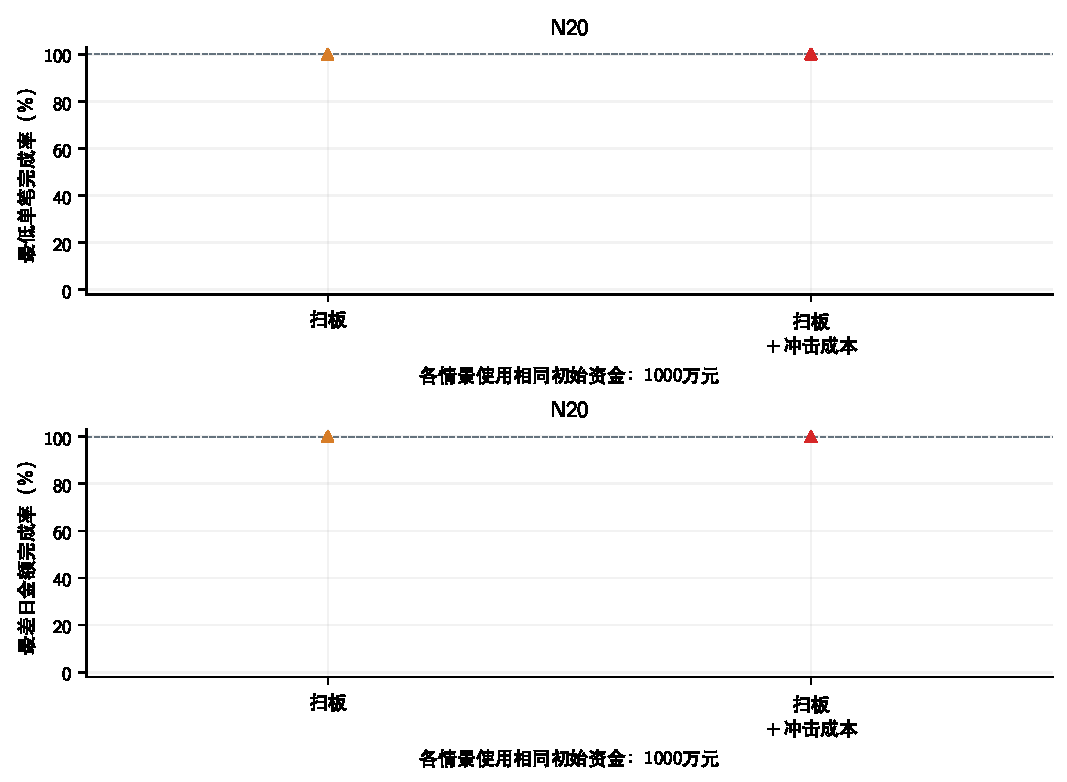
\includegraphics[width=\linewidth]{figures/capital_completion.pdf}
\caption{最低单笔完成率与最差交易日金额完成率。颜色区分执行情景；圆点通过、叉号未通过、三角待核实。不同情景分别回放，不能把账户数当作资金档数。}\end{figure}
\section*{额外冲击成本与账户结果}这项成本用于测试可见盘口之外的额外交易代价，在每次成交前占用现金，并影响可买数量和卖出净收入。成交价格仍是实际盘口档价或扫板官方限价，背景估值价格不变。扫板的100\%后续有效新增量可用仍是情景假设，新增成本没有复原真实排队或其他交易者反应。\[\Delta C=k\,\frac{(X+\Delta X)^{3/2}-X^{3/2}}{\sqrt{M}},\qquad k=\frac{b}{10000\sqrt{0.1}}.\]$\Delta C$是本次拟成交的额外成本，单位为元；$X$是当天此前同账户、同证券、同方向已成交金额；$\Delta X$是本次拟成交额；$M$是本次成交前已经观察到的当日市场累计成交额，三者单位均为元。$b$以基点计，1基点等于万分之一；$k$把基点参数换成公式所需系数。本报告参数b为5基点，表示在固定M下累计执行额占已知市场额10\%时的累计平均额外成本，属于未校准的敏感性假设。\par 示例：设$X=0$元、$\Delta X=100$万元、$M=1000$万元、$b=5$基点。本次成交额占当时已知市场额的10\%，额外成本为$1000000\times5/10000=500$元。这是公式算例，不是公司实盘估计。

同一天拆分子单不清空累计金额。市场累计额随时间增加时，后续成本随新观测计算，之前费用不退回；新交易日重新累计。盘中不使用未来全天成交额。\begin{figure}[H]\centering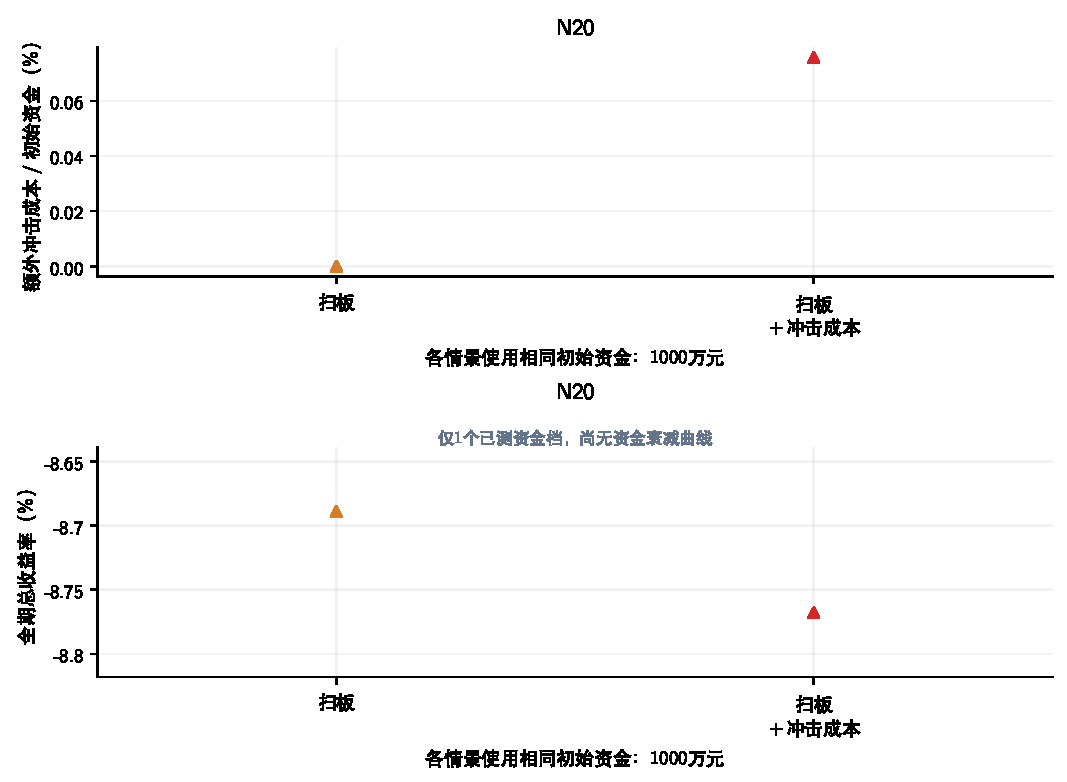
\includegraphics[width=\linewidth]{figures/capital_impact.pdf}\caption{额外冲击成本占初始资金及冲击后的全期模型收益。不同账户路径的收益差不等于直接冲击费用；未设置经济容量阈值。}\end{figure}\begin{table}[H]\centering\scriptsize\begin{tabular}{lllrrrr}\toprule N & 情景 & 资金 & 盘口成本(万) & 扫板价差(万) & 额外冲击(万) & 佣金税费(万)\\\midrule N20 & 扫板 & 1000万元 & 待核 & 待核 & 未启用 & 0 \\
N20 & 扫板＋冲击成本 & 1000万元 & 11.2 & 0.07 & 0.76 & 0 \\\bottomrule\end{tabular}\end{table}盘口成本和扫板价差相对当时背景中价计量，已包含于成交金额；额外冲击与佣金税费独立计入现金。表列各组最低已测资金，全部资金见图源表。\section*{原计划完成时间}以原计划日的固定正数量需求为分母，30／60分钟均为交易分钟，扣除午休。后续记录不新增原日计划，也不改写原日结果。未完成计划和缺时间证据的计划保留在分母；待定量目标另列在随附表。下表列各组最低已测资金，全部资金及已完成计划耗时分位数见图源表。\begin{table}[H]\centering\scriptsize\begin{tabular}{lllrrrrr}\toprule N & 情景 & 资金 & 正计划 & 30分全成 & 60分全成 & 当日未成 & 时间待核\\\midrule N20 & 扫板 & 1000万元 & 11506 & 11502 & 11505 & 0 & 0 \\
N20 & 扫板＋冲击成本 & 1000万元 & 11505 & 11501 & 11504 & 0 & 0 \\\bottomrule\end{tabular}\end{table}案例1为N20的扫板＋冲击成本账户，资金1000万元，2024-01-11原计划2800股／份，当日实际成交2800，剩余0。该计划没有已保存的扫板触发证据。额外模型冲击成本0.74元，单独进入现金，不改变官方成交价格。\begin{figure}[H]\centering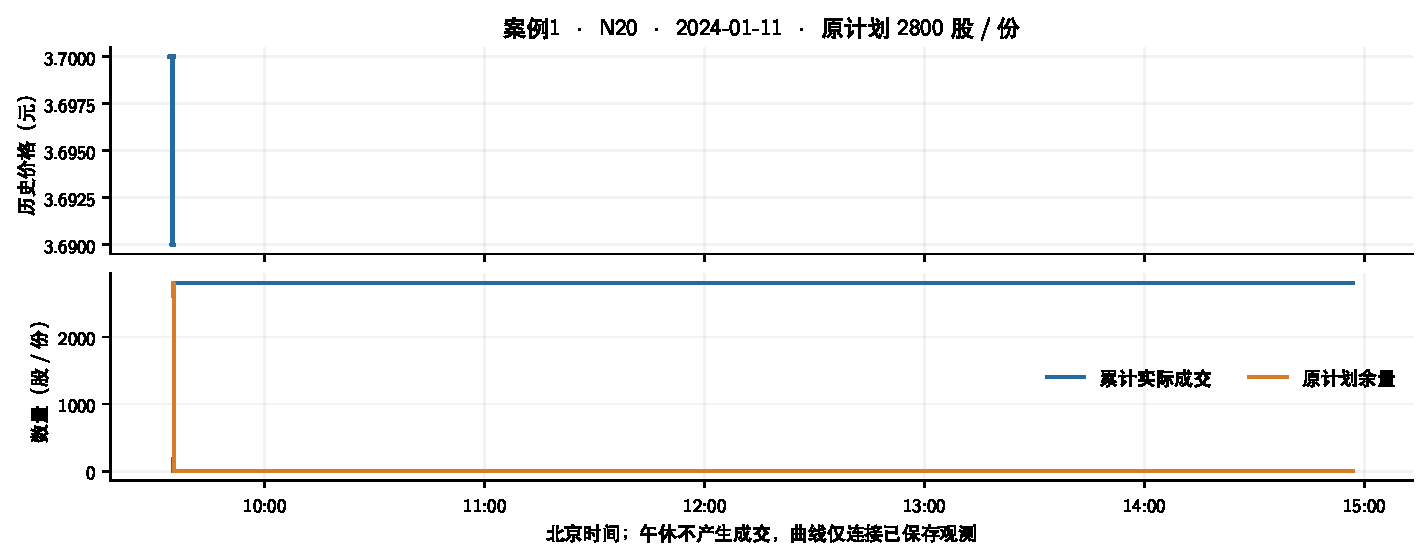
\includegraphics[width=.85\linewidth]{figures/intraday_1.pdf}\caption{实际历史观测与该账户的原计划执行。案例说明执行过程，不代表发生频率；不同情景各用自己的计划与账户路径。}\end{figure}案例2为N20的扫板＋冲击成本账户，资金1000万元，2024-01-11原计划500股／份，当日实际成交500，剩余0。扫板首次触发于09:35:00。其中实际扫板成交500股／份。额外模型冲击成本0.08元，单独进入现金，不改变官方成交价格。\begin{figure}[H]\centering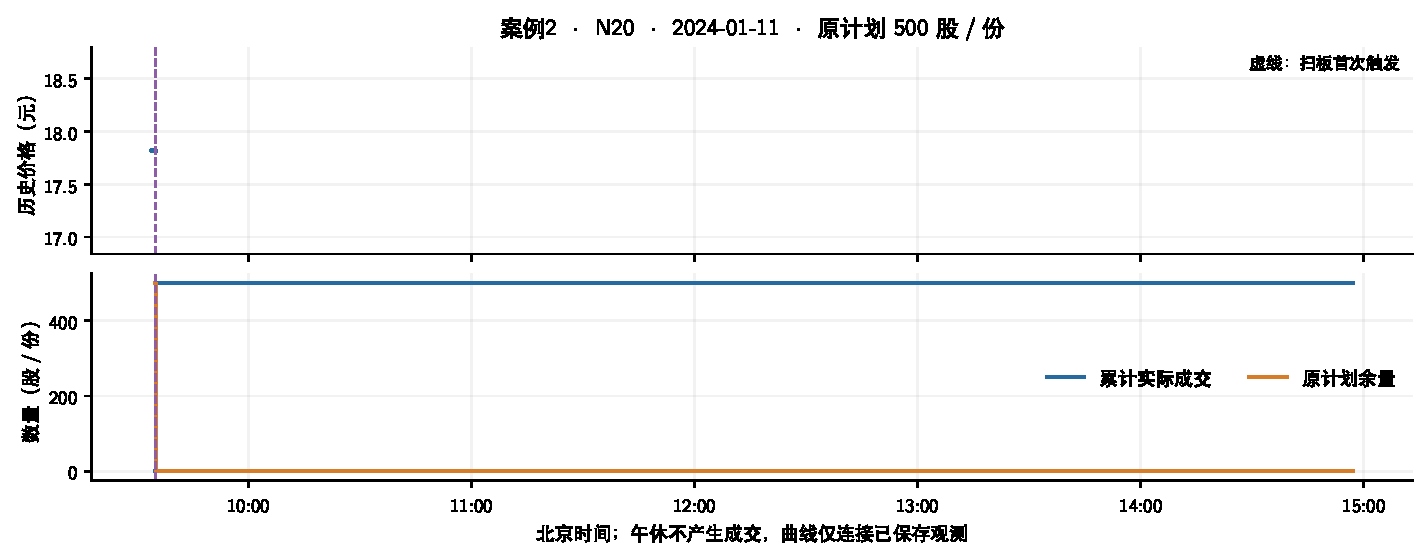
\includegraphics[width=.85\linewidth]{figures/intraday_2.pdf}\caption{实际历史观测与该账户的原计划执行。案例说明执行过程，不代表发生频率；不同情景各用自己的计划与账户路径。}\end{figure}

\end{document}
